\documentclass{article}
\usepackage[margin=1in]{geometry}
\usepackage{url}
\usepackage{booktabs}
\usepackage{forest}
\usepackage{tabu}
\usepackage{listings}
\usepackage{amsmath}
\usepackage{amsfonts}
\usepackage{float}
\usepackage{color}
\usepackage{multicol}
\usepackage[colorlinks = true,
            linkcolor = blue,
            urlcolor  = blue,
            citecolor = blue,
            anchorcolor = blue]{hyperref}
\usepackage{subfig}
\usepackage[font=small,labelfont=bf]{caption} 

\newcommand{\MYhref}[3][blue]{\href{#2}{\color{#1}{#3}}}%

\definecolor{dkgreen}{rgb}{0,0.6,0}
\definecolor{gray}{rgb}{0.5,0.5,0.5}
\definecolor{mauve}{rgb}{0.58,0,0.82}

\lstset{frame=tb,
  language=Java,
  aboveskip=3mm,
  belowskip=3mm,
  showstringspaces=false,
  columns=flexible,
  basicstyle={\small\ttfamily},
  numbers=none,
  numberstyle=\tiny\color{gray},
  keywordstyle=\color{blue},
  commentstyle=\color{dkgreen},
  stringstyle=\color{mauve},
  breaklines=true,
  breakatwhitespace=true,
  tabsize=3
}

\title{Compute Bound CPU Matrix Multiplication}
\author{Rami Pellumbi\thanks{M.S., Statistics \& Data Science}}
\date{\today}

\begin{document}

\maketitle
\tableofcontents

\newpage 

\section{Introduction}
Inspired by a YouTube video \MYhref{https://www.youtube.com/watch?v=QGYvbsHDPxo}{`Adding Nested 
Loops Makes this Algorithm 120x FASTER'}, this project aims to implement a highly optimized
matrix multiplication algorithm on CPUs. The video demonstrates how the performance of a
naive matrix multiplication algorithm can be improved by simply reordering the loops and 
implementing a blocking strategy. The video also highlights the importance of memory access
patterns in matrix multiplication.

\

\noindent Matrix multiplication is a cornerstone operation in numerous computational fields,
ranging from scientific computing to machine learning. At its core, the operation 
involves the element-wise multiplication and summation of elements across two matrices 
to produce a third matrix. The theoretical simplicity of this operation belies its 
computational complexity, particularly when dealing with large matrices. 
Matrix multiplication scales with the size of the input matrices, often resulting 
in a significant computational challenge for even modern day processors. 
This challenge is accentuated by the fact that CPUs, with their limited number 
of cores and sequential processing capabilities, are often outperformed by GPUs in 
parallelizable tasks like matrix multiplication. However, understanding and optimizing 
matrix multiplication on CPUs is crucial, as CPUs are more universally accessible 
and are often the primary computing resource available in many environments.

\ 

\noindent The difficulty in optimizing matrix multiplication on CPUs stems from several factors. 
First, the computational intensity: as the size of the matrices increases, 
the number of calculations grows cubically, leading to a steep increase in the 
required computational resources. Second, memory access patterns play a critical role: as the 
size of the matrices increase, the total memory accesses increase quadratically.
Efficient matrix multiplication algorithms must minimize cache misses and effectively utilize 
the CPU cache hierarchy. This is challenging due to the non-contiguous memory access 
patterns inherent in naive matrix multiplication. 

\

\noindent The current state of the art in matrix multiplication optimization are built 
on top of Basic Linear Algebra Subprograms (BLAS). The magic of BLAS lies in its ability 
to significantly optimize these computationally intensive operations. 
These routines are meticulously engineered to exploit the underlying architecture of CPUs to their fullest, 
leveraging techniques such as loop unrolling, blocking for cache, and efficient use of SIMD instructions. 
These optimizations allow BLAS to achieve performance levels that are often an order 
of magnitude faster than naive implementations. This project started as 
`investigate this videos claims' and ended with the goal of matching the performance 
of Intel's Math Kernel Library (MKL) implementation of \texttt{dgemm}: a highly optimized 
matrix multiplication routine for double precision matrices. 

\section{CPU Specifications}\label{SEC:CPU-SPECS}
The Intel Xeon(R) Platinum 8268 CPU in the Cascade Lake family is used for profiling. 
The processor has 24 cores, each with 2 threads, for a total of 48 threads and operates 
at 3.5GHz. With 512-bit floating-point vector registers and two floating-point 
functional units, each capable of Fused Multiply-Add (FMA), a Cascade Lake core can 
deliver 32 double-precision floating-point operations per cycle.\footnote{\MYhref{https://www.nas.nasa.gov/hecc/support/kb/cascade-lake-processors_579.html}{https://www.nas.nasa.gov/hecc/support/kb/cascade-lake-processors\_579.html}}
This brings the theoretical peak performance of the CPU (with no virtual threads enabled) to 
\begin{align*}
    3.5\ \texttt{GHz} * 24\ \texttt{cores} * 32\ \frac{\texttt{FLOPs}}{\texttt{core}} = 2688\ \texttt{GFLOPs}.
\end{align*}
For a single core of the CPU, this is of course
\begin{align*}
    3.5\ \texttt{GHz} * 32\ \frac{\texttt{FLOPs}}{\texttt{core}} = 112 \ \texttt{GFLOPs}. 
\end{align*}

\subsubsection*{Cache Specifications}
\paragraph{L1}
Each of the 24 cores has a 32K \texttt{L1d} cache. It is 8-way set associative, utilizes a write-back policy, and is dedicated to data storage. The cache line size is 64 bytes.
Moreover, each core has a 32K \texttt{L1i} cache. It is 8-way set associative, utilizes a write-back policy, and is dedicated to instruction storage. The cache line size is 64 bytes.

\paragraph{L2}
Each of the 24 cores has a 1024K \texttt{L2} cache. It is 16-way set associative, utilizes a write-back policy, and handles both instructions and data.

\paragraph{L3}
There is a single 36608K \texttt{L3} cache shared across all cores. It is 11-way set associative, utilizes a write-back policy, and handles both instructions and data.

\subsubsection*{Memory Details}
The processor has a maximum theoretical memory bandwidth of 131.13 \texttt{GiB/s}. 
Each \texttt{double} takes up 8 bytes of memory. This means that the CPU memory bandwidth is 
\begin{align*}
    \texttt{140.8GB/s} \cdot \frac{\texttt{double}}{\texttt{8B}} = 17.6\ \texttt{GFlops/s}
\end{align*}
per socket. 

\section{The Problem}

Matrix multiplication inherently becomes compute-bound and delves into the 
nuances of compute and memory access that escalate as matrix sizes scale.

\subsection{Compute-Bound Nature of Matrix Multiplication}

The essence of a compute-bound task lies in its primary limitation being the 
processing power of the CPU rather than I/O or memory speeds. As illustrated in the Section \ref{SEC:CPU-SPECS}, the theoretical peak performance of the CPU is
2688 \texttt{GFLOPs}. However, the theoretical peak memory bandwidth is only 17.6 \texttt{GFlops/s};
152x slower. Thus, any task that requires more than 152 CPU cycles per memory access (in a 24 core program) will be
compute bound (and any task requiring less than 152 CPU cycles per memory access is memory bound).\footnote{
    For the single core case, this reduces to about 6 CPU cycles per memory access.
}

\

\noindent Matrix multiplication, especially for large matrices, is intensely compute-intensive. 
The standard algorithm for matrix multiplication involves three nested loops, 
iterating over the rows and columns of the input matrices. 
For two matrices of size \( N \times N \), this results in a computational complexity of 
\( O(N^3) \). Each element in the resultant matrix is computed by taking the dot product of 
a row from the first matrix and a column from the second, involving \( N \) 
multiplications and \( N-1 \) additions. As \( N \) increases, the number of 
arithmetic operations grows cubically, making the task increasingly compute-bound.

\subsection{Memory Access Patterns and Their Impact}

Apart from the computational intensity, memory access patterns significantly 
influence the performance of matrix multiplication algorithms. As matrix sizes grow, 
the memory footprint of these matrices also expands, often surpassing the size of the CPU 
caches, e.g., multiplying 2 $N \times N$ double precision matrices requires
\begin{align*}
    3 * N * N * 8 \texttt{ bytes},
\end{align*}
which exceeds the size of the \texttt{L3} cache at just $N = 1250$.
This mismatch leads to frequent cache misses and the necessity to fetch 
data from the slower main memory, introducing latency.

\

\noindent The non-contiguous memory access patterns in matrix multiplication exacerbate this issue. 
Accessing elements row-wise in one matrix and column-wise in another leads to strided accesses, 
which are inefficient for cache utilization. In large matrices, these strided accesses mean that 
the processor cannot effectively prefetch data, leading to increased cache misses and memory 
latency.

\subsection{The Challenge of Optimizing for Larger Matrices}

Optimizing matrix multiplication for larger matrices thus becomes a dual challenge: managing the cubic growth in computational requirements and minimizing memory latency due to inefficient access patterns. Effective optimization requires a nuanced understanding of both the computational architecture and the memory hierarchy of CPUs. Techniques like loop reordering, tiling, or blocking, which aim to maximize data locality and cache utilization, become critical. However, these techniques must be meticulously tailored to the specific architecture, as the optimal configuration can vary significantly based on factors like cache size, cache line size, and the number of cores.

\section{Approach 1: Keep it Serial}
The first batch of programs focused on optimizing a serial matrix multiplication algorithm.
First, the naive algorithm was implemented. Then, the loops were reordered to improve cache performance.
Finally, a blocking strategy was implemented to further improve cache performance. All 
algorithms were written to compute $C = A \times B$, where $A$ is an $N \times P$ 
matrix and $B$ is a $P \times M$ matrix. The resultant matrix $C$ is of course $N \times M$. 
All matrix multiplies were compared against the BLAS implementation of matrix multiplication 
(\texttt{dgemm}) for correctness. Unless otherwise stated, matrices are stored in row-major order.

\subsection{The Naive Algorithm}
The naive algorithm is the most straightforward implementation of matrix multiplication. 
It uses the standard \texttt{ijk} access pattern and is implemented as follows:
\begin{lstlisting}
for (int i = 0; i < N; i++)
{
    int iA = i * P; // get to index for start of row i
    for (int j = 0; j < M; j++)
    {
        int iC = i * M + j; // row i column j of C

        double cvalue = 0.;
        for (int k = 0; k < P; k++)
        {
            int jB = k * M + j;
            // row i column k of A multiplied with row k column j of B
            C[iC] += A[iA + k] * B[jB];
        }
    }
}
\end{lstlisting}
\noindent This is terribly inefficient for a few reasons:
\begin{enumerate}
    \item The innermost loop performs 2 loads and 1 store.
    \item $B$ is accessed column-wise (\(k * M + j\)). This access pattern is inefficient in a row-major storage system since elements are not contiguous in memory. This leads to a compulsory miss rate of 1.\footnote{
        A compulsory miss refers to the cache miss that occurs when the first access to a block is not in the cache. The cache line size is 64 bytes. Thus, for access 
        to a consecutive doubles (8 bytes), the compulsory miss rate is 8/64 = 0.125 (in ideal conditions).
    }
    \item There is poor temporal locality - only somewhat utilized in accessing elements of A and C, as the same elements of these matrices are accessed multiple times within the inner loops. Each has a compulsory miss rate of 0.125.
\end{enumerate}
The code is so ill performing that only select matrix sizes were evaluated. The 
results are shown in Table \ref{TAB:NAIVE-RESULTS}. The results are in seconds and
are the average of 3 runs. The MKL libraries \texttt{dgemm} implementation is included for comparison. 
\begin{table}[H]
    \centering
    \caption{ijk Access Pattern Mean Performance (s)}
    \begin{tabular}[t]{rrrrr}
    \toprule
    N & P & M & Mean Time & Mean Blas Time\\
    \midrule
    1024 & 1024 & 1024 & 1.691 & 0.053\\
    \addlinespace
    2048 & 2048 & 2048 & 16.157 & 0.274\\
    \bottomrule
    \end{tabular}
    \label{TAB:NAIVE-RESULTS}
\end{table}
\noindent The Intel MKL \texttt{dgemm} implementation is 32x faster than the naive implementation for $N = 1024$ and 59x faster for $N = 2048$. The naive implementation is clearly not scalable.

\subsection{Loop Reordering}
The next step was to attempt to remedy the access pattern inefficiencies by reordering the loops. The 
\texttt{kij} access pattern was chosen. This pattern is implemented as follows:
\begin{lstlisting}
for (int k = 0; k < P; k++)
{
    for (int i = 0; i < N; i++)
    {
        int iA = i * P + k; // get row i column k of A for reuse
        double r = A[iA];
        for (int j = 0; j < M; j++)
        {
            int iB = k * M + j; // row k column j of B
            int iC = i * M + j; // row i column j of c
            C[iC] += r * B[iB];
        }
    }
}
\end{lstlisting}
\noindent The \texttt{kij} access pattern offers significant improvements over the \texttt{ijk} pattern for matrix multiplication, 
primarily due to its more efficient use of the CPU cache. The outermost loop iterates over the $k$-dimension (columns of $A$), followed by the $i$ (rows of $A$) and $j$ (columns of $B$) dimensions. 
This restructuring has significant implications for memory access patterns.
\begin{enumerate}
    \item The compulsory miss rate of $A$ is reduced to zero (as opposed to 0.125 in the \texttt{ijk} pattern). 
    \item The compulsory miss rate of $B$ is reduced to 0.125 (as opposed to 1 in the \texttt{ijk} pattern).
    \item The compulsory miss rate of $C$ remains at 0.125 (as opposed to 0.125 in the \texttt{ijk} pattern).
\end{enumerate}
The results are shown in Table \ref{TAB:REORDERED-RESULTS}. The results are in seconds and
are the average of 3 runs. The MKL libraries \texttt{dgemm} implementation is included for comparison.
\begin{table}[H]
    \centering
    \caption{kij Access Pattern Mean Performance (s)}
    \begin{tabular}[t]{rrrrr}
    \toprule
    N & P & M & Mean Time & Mean Blas Time\\
    \midrule
    1024 & 1024 & 1024 & 0.356 & 0.053\\
    \addlinespace
    1024 & 1024 & 8192 & 5.230 & 0.297\\
    \addlinespace
    8192 & 1024 & 8192 & 46.062 & 2.042\\
    \addlinespace
    8192 & 8192 & 1024 & 39.845 & 1.949\\
    \addlinespace
    8192 & 8192 & 8192 & 370.106 & 15.499\\
    \bottomrule
    \end{tabular}
    \label{TAB:REORDERED-RESULTS}
\end{table}
\noindent We see that for the one overlapping matrix size ($N = P = M = 1024$), the \texttt{kij} access pattern is $4.75\times$ faster than the \texttt{ijk} access pattern. 
The Intel MKL \texttt{dgemm} implementation still far outperforms the \texttt{kij} access pattern, but the gap has narrowed significantly. 

\ 

\noindent It is time to take a step back and consider CPU utilization. Figure \ref{FIG:CPU-UTILIZATION} shows the performance 
in terms of GFLOPs/s for the \texttt{kij} access pattern juxtaposed to the Intel MKL \texttt{dgemm} implementation. 
\begin{figure}[H]
    \centering
    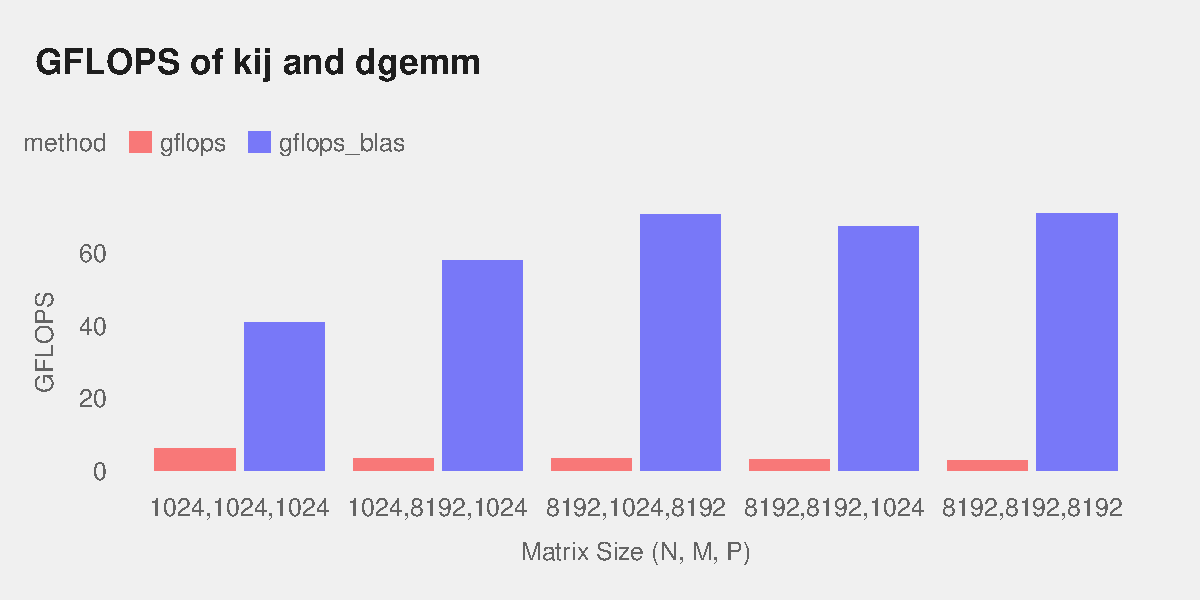
\includegraphics[width=0.8\textwidth]{../../project/out/kij-gflops.pdf}
    \caption{Performance of \texttt{kij} Access Pattern vs. Intel MKL \texttt{dgemm} Implementation in GFLOPs/s}
    \label{FIG:CPU-UTILIZATION}
\end{figure}
\noindent It is immediately evident that the \texttt{kij} access pattern is not utilizing the CPU to its fullest. 
Indeed, what should be a compute bound task is memory bound. We need to dig deeper.

\subsection{Tiled Matrix Multiplication}
This brings us to the video, which introduces tiling as a strategy to improve cache performance. 
This technique involves subdividing the input matrices into smaller blocks or sub-matrices, 
which are then processed individually. The key advantage of matrix tiling lies in its 
ability to significantly reduce cache misses by ensuring that the working set of data — 
the subset of the matrices actively being used in computations — fits into the faster, 
but smaller, levels of the CPU cache. By processing these smaller blocks, 
the algorithm can keep a block of each matrix in the cache for the duration of 
the computation of a sub-matrix of the result, thereby minimizing the costly memory 
accesses to the slower main memory. 

\ 

\noindent This is particularly effective for large matrices where the entire matrix 
cannot be stored in the cache at once. Tiling optimizes the memory hierarchy usage, 
making efficient use of the CPU's cache to speed up the computation, and is especially 
crucial for larger matrices where the non-tiled approach leads to frequent cache evictions. 
As such, tiling is a natural next step in our optimization journey, 
aiming to bridge the gap between theoretical and practical performance on our CPU.

\

\noindent The blocking strategy takes our initial program and makes the realization that 
\begin{align*}
    C[i][j] = \sum_{k = 0}^P A[i][k] * B[k][j]
\end{align*}
is functionally equivalent to 
\begin{align*}
    C[i][j] = \sum_{b = 0}^L \sum_{k = 0}^{P / L} A[i]\bigg[\frac{bP}{L}\bigg] * B\bigg[\frac{bP}{L}\bigg][j] 
\end{align*}
Under the assumption that our matrix dimension $M, N, P$ are multiples of $L$, we can write 
our program as 6 nested loops:
\begin{lstlisting}
for (int ii = 0; ii < N; ii += BLOCK_SIZE)
{
    for (int jj = 0; jj < M; jj += BLOCK_SIZE)
    {
        for (int kk = 0; kk < P; kk += BLOCK_SIZE)
        {
            for (int i = ii; i < ii + BLOCK_SIZE; i++)
            {
                iA = i * P;
                for (int j = jj; j < jj + BLOCK_SIZE; j++)
                {
                    iC = i * M + j;
                    for (int k = kk; k < kk + BLOCK_SIZE; k++)
                    {
                        jB = k * M + j;
                        C[iC] -= A[iA + k] * B[jB];
                    }
                }
            }
        }
    }
}
\end{lstlisting}
This is an overly simplistic approach and up to now, we have not made any assumptions 
on our matrix dimensions. In the spirit of keeping things general, we make the realization 
that we can think of our multiplication of $A$ and $B$ as the multiplication 
\begin{align*}
    \begin{bmatrix}
        A_{1} & A_{2} \\ A_{3} & A_{4}
    \end{bmatrix}
    \begin{bmatrix}
        B_{1} & B_{2} \\ B_{3} & B_{4}
    \end{bmatrix},
\end{align*}
where $A_{1}$ and $B_{1}$ are multiples of $L$ and the remaining blocks are the residuals. 
Thus, the above loop handles $A_1 B_1$ and we can handle the residual case by including cleanup loops
to multiply the remaining blocks. The details are observable in the code in \texttt{t3-serial-blocking.c}. 
The performance of this algorithm is shown in Table \ref{TAB:TILED-RESULTS}. The results are in seconds and
are the average of 3 runs. The MKL libraries \texttt{dgemm} implementation is included for comparison.
\begin{table}[H]
    \centering
    \caption{Blocked Access Pattern Mean Performance (s)}
    \begin{tabular}[t]{rrrrrrr}
    \toprule
    N & P & M & Block Size & Mean blocked Time & Mean kij Time & Mean Blas Time\\
    \midrule
    1024 & 1024 & 1024 & 16 & 0.305 & 0.356 & 0.053\\
    \addlinespace
    1024 & 1024 & 8192 & 16 & 3.244 & 5.230 & 0.297\\
    \addlinespace
    8192 & 1024 & 8192 & 16 & 25.632 & 46.062 & 2.042\\
    \addlinespace
    8192 & 8192 & 1024 & 16 & 27.166 & 39.845 & 1.949\\
    \addlinespace
    8192 & 8192 & 8192 & 16 & 215.646 & 370.106 & 15.499\\
    \bottomrule
    \end{tabular}
    \label{TAB:TILED-RESULTS}
\end{table}
\noindent We observe the blocking strategy is significantly faster than the naive and reordering strategies.
Still, the MKL libraries \texttt{dgemm} implementation is much faster than our implementation on a single thread. 
We are still underutilizing the cache. To remedy this, we consider transposing the matrix $B$ 
before the multiply. This allows for more efficient loading of $A$ and $B$ in the inner loops 
allowing the compiler to optimize the code better, e.g., via SIMD instructions. 
The results are shown in Table \ref{TAB:TILED-TRANSPOSED-RESULTS}. 
\begin{table}[H]
    \centering
    \caption{Blocked Access Pattern Mean Performance (s)}
    \begin{tabular}[t]{rrrrrrr}
    \toprule
    N & P & M & Block Size & Mean blocked Time & Mean kij Time & Mean Blas Time\\
    \midrule
    1024 & 1024 & 1024 & 16 & 0.205 & 0.356 & 0.053\\
    \addlinespace
    1024 & 1024 & 8192 & 16 & 1.817 & 5.230 & 0.297\\
    \addlinespace
    8192 & 1024 & 8192 & 16 & 13.966 & 46.062 & 2.042\\
    \addlinespace
    8192 & 8192 & 1024 & 16 & 21.377 & 39.845 & 1.949\\
    \addlinespace
    8192 & 8192 & 8192 & 16 & 149.600 & 370.106 & 15.499\\
    \bottomrule
    \end{tabular}
    \label{TAB:TILED-TRANSPOSED-RESULTS}
\end{table}
\noindent The block size for 16 is shown only as other block sizes performed significantly worse.

\subsection{Blocking Cache Analysis}
Each of $A$ and $B$ is partitioned into $L \times L$ chunks. 
The innermost $(i,j,k)$ loops multiply a $L \times L$ chunk of $A$ with a
$L \times L$ chunk of $B$ and accumulates the 
result in a $L \times L$ chunk of $C$.

\

\noindent Assuming the dimensions are a multiple of block size $L$, with a block size of $L = 16$, we have 
\begin{align*}
    16 * 16 * 8 * 3 \ \texttt{bytes} = 6144\ \texttt{bytes},
\end{align*}
and so all of our matrix chunks can reside in the \texttt{L1} cache. We anticipate 
$L^2 / 8 = 32$ misses per chunk and thus $32 * 3 = 96$ misses per chunk iteration. 
Thus, the blocking strategy has a total of 
\begin{align*}
    \frac{M}{L} \cdot \frac{N}{L} \cdot \frac{P}{L} \cdot \frac{3 L^2}{8} = \frac{3 \cdot M \cdot N \cdot P}{8 * L} = \frac{3M\cdot N \cdot P}{128}\ \texttt{misses}.
\end{align*}
Compared to the \texttt{kij} algorithm, which had $0.25$ misses per iteration for a total miss count of $M\cdot N \cdot P / 4$, it 
is evident we are making significant progress in cache utilization.

\

\noindent We are still nowhere near the theoretical peak performance of the CPU for a single thread and we are 
out of ideas from the video when it comes to serial code. We move on to multithreading 
to exhaust the videos suggestions, before we attempt to really understand the beast that is \texttt{dgemm}.

\section{Approach 2: Leveraging Multithreading}

To leverage multithreading, we utilize OpenMP: an industry standard API for 
shared-memory parallelism. We distribute the matrix multiplication workload 
across the cores of the CPU, significantly reducing the computation time. 
It was discovered that Intel's MKL library only makes use of the number of 
threads allotted to the program. Thus, as the \texttt{OMP\_NUM\_THREADS} environment variable is varied, 
the performance of the MKL libraries \texttt{dgemm} implementation varies accordingly 
- something that was not expected and made \texttt{dgemm} feel even more out of reach.

\subsection{OpenMP}
The first thing to do is just parallelize where we left off in the serial code. This is 
done simply with the \texttt{\#pragma omp parallel for} directive on the outermost loop 
of the multiply. The results are shown in Table \ref{TAB:OMP-RESULTS}.
\begin{table}[H]
    \centering
    \caption{OMP Mean Performance - 24 cores (s)}
    \begin{tabular}[t]{rrrrrr}
    \toprule
    N & P & M & Block Size & Mean Time & Mean Blas Time\\
    \midrule
    1000 & 1000 & 1000 & 16 & 0.013 & 0.024\\
    \addlinespace
    1024 & 1024 & 1024 & 16 & 0.020 & 0.024\\
    \addlinespace
    1024 & 1024 & 8192 & 16 & 0.208 & 0.037\\
    \addlinespace
    8192 & 1024 & 8192 & 16 & 0.999 & 0.128\\
    \addlinespace
    8192 & 8192 & 1024 & 16 & 1.096 & 0.130\\
    \addlinespace
    8192 & 8192 & 8192 & 16 & 10.227 & 0.756\\
    \addlinespace
    9600 & 9600 & 9600 & 16 & 8.930 & 1.072\\
    \bottomrule
    \end{tabular}
    \label{TAB:OMP-RESULTS}
\end{table}
\noindent For small matrices, MKL's \texttt{dgemm} does not benefit much from multithreading.
However, for larger matrices, the performance of the MKL implementation improves significantly
more than our implementation, e.g., for $M = N = P = 8192$, the MKL implementation is 20x faster than 
its serial counterpart whereas our blocked implementation is only 15x faster. 

\subsection{Fixing False Sharing}
One problem our blocked implementation suffers from in the multithreading case is false sharing. In a shared memory 
program, cache coherence protocols guarantee the consistency between data residing in the various levels of 
cache and main memory. In certain programs, cache coherence protocols can lead to a significant performance
degredation. Specifically, if the same cache line is continuously accessed or modified by different threads, forcing the cache 
coherence protocol to evict and reload it in rapid successions, we say that the threads are experiencing false sharing.\footnote{I 
was unsure how to cite this, but this reasoning is from Hager's 2nd edition of `Introduction to High Performance Computing for Scientists and Engineers'.}

\

\noindent There are a few different ways to fix false sharing, the most simple of which is to privatize the data 
each thread is accessing. At the entry point of the parallel region, we make local $L \times L$ copies 
of the blocks of $A$, $B$, and $C$ that each thread will be accessing. This gives each thread 
access to the appropriate matrix block on its own stack space, eliminating the interference from cache coherence.

\

\noindent Along with this, we also utilize the more efficient \texttt{kij} access pattern and get rid of transposing the 
matrix $B$. To implement, we first declare the private blocks of $A$, $B$, and $C$ with the \texttt{threadprivate} directive:
\begin{lstlisting}
#define BLOCK_SIZE 32
alignas(64) static double blockA[BLOCK_SIZE][BLOCK_SIZE];
alignas(64) static double blockB[BLOCK_SIZE][BLOCK_SIZE];
alignas(64) static double blockC[BLOCK_SIZE][BLOCK_SIZE]; 
#pragma omp threadprivate(blockA, blockB, blockC)
\end{lstlisting}
The local blocks are aligned on 64-byte boundaries so that a cache line will have exactly 8 doubles in it (maximizing cache utilization).
Now that each thread has its own local copies of the blocks, we can simply copy the blocks into the local
copies at the beginning of the parallel region and copy them back into the global $C$ at the end of the parallel region:
\newpage
\begin{lstlisting}
#pragma omp parallel default(none) shared(N, P, M, A, B, C) private(iA, jB, iC)
{
    #pragma omp for schedule(runtime)
    for (size_t ii = 0; ii < N; ii += BLOCK_SIZE)
    {
        for (size_t jj = 0; jj < M; jj += BLOCK_SIZE)
        {
            // clear blockC as infrequently as needed
            for (size_t i = 0; i < BLOCK_SIZE; i++)
                for (size_t j = 0; j < BLOCK_SIZE; j++) blockC[i][j] = 0.;

            for (size_t kk = 0; kk < P; kk += BLOCK_SIZE)
            {
                // Copy blocks of A and B into blockA and blockB
                for (size_t i = 0; i < BLOCK_SIZE; i++)
                {
                    iA = (ii + i) * P + kk;
                    jB = (kk + i) * M + jj;
                    for (size_t j = 0; j < BLOCK_SIZE; j++)
                    {
                        blockA[i][j] = A[iA + j];
                        blockB[i][j] = B[jB + j];
                    }
                }

                // Perform block multiplication on private blocks
                for (size_t k = 0; k < BLOCK_SIZE; k++)
                {
                    for (size_t i = 0; i < BLOCK_SIZE; i++)
                    {
                        double r = blockA[i][k];
                        for (size_t j = 0; j < BLOCK_SIZE; j++)
                        {
                            blockC[i][j] += r * blockB[k][j];
                        }
                    }
                }
            }

            // copy blockC back into C
            for (size_t i = 0; i < BLOCK_SIZE; i++)
            {
                iC = (ii + i) * M + jj;
                for (size_t j = 0; j < BLOCK_SIZE; j++)
                {
                    C[iC + j] -= blockC[i][j];
                }
            }
        }
    }
}
\end{lstlisting}
The results of this approach are in the below Table \ref{TAB:OMP-RESULTS-PRIVATIZED}.
\begin{table}[H]
    \centering
    \caption{OMP Privatized Data Mean Performance - 24 cores (s)}
    \begin{tabular}[t]{rrrrrr}
    \toprule
    N & P & M & Block Size & Mean Time & Mean Blas Time\\
    \midrule
    1024 & 1024 & 1024 & 32 & 0.008 & 0.024\\
    \addlinespace
    1024 & 1024 & 8192 & 32 & 0.082 & 0.037\\
    \addlinespace
    8192 & 1024 & 8192 & 32 & 0.455 & 0.128\\
    \addlinespace
    8192 & 8192 & 1024 & 32 & 0.512 & 0.130\\
    \addlinespace
    8192 & 8192 & 8192 & 32 & 3.889 & 0.756\\
    \addlinespace
    9600 & 9600 & 9600 & 32 & 6.822 & 1.072\\
    \bottomrule
    \end{tabular}
    \label{TAB:OMP-RESULTS-PRIVATIZED}
\end{table}
\noindent This was a significant improvement. For $M = N = P = 8192$, the performance of our implementation
improved $2.6\times$ over the non-privatized data approach, and all across the board we see greater than $2\times$ improvement. 

\

\noindent It must be noted that this approach assumed that the matrix dimensions were multiples of the block size. The general 
solution was also implemented, but the performance took a small hit since at the beginning of each multiply the matrices must 
be padded to be multiples of the block size. The results are shown in Table \ref{TAB:OMP-RESULTS-PRIVATIZED-GENERAL} and we 
note the still much improved performance over the non privatized case.
\begin{table}[H]
    \centering
    \caption{OMP Privatized Data Mean Performance (General) - 24 cores (s)}
    \begin{tabular}[t]{rrrrrr}
    \toprule
    N & P & M & Block Size & Mean Time & Mean Blas Time\\
    \midrule
    1000 & 1000 & 1000 & 32 & 0.013 & 0.024\\
    \addlinespace
    1024 & 1024 & 1024 & 32 & 0.013 & 0.024\\
    \addlinespace
    1024 & 1024 & 8192 & 32 & 0.104 & 0.037\\
    \addlinespace
    8192 & 1024 & 8192 & 32 & 0.496 & 0.128\\
    \addlinespace
    8192 & 8192 & 1024 & 32 & 0.674 & 0.130\\
    \addlinespace
    8192 & 8192 & 8192 & 32 & 4.177 & 0.756\\
    \addlinespace
    9600 & 9600 & 9600 & 32 & 7.225 & 1.072\\
    \bottomrule
    \end{tabular}
    \label{TAB:OMP-RESULTS-PRIVATIZED-GENERAL}
\end{table}
\noindent A more clever solution would only make copies of the blocks that are not multiples of the block size, but this was not implemented.

\subsection{Recapping Progress}
Up to now, we have observed how tiling, multithreading, privatizing data to threads, and efficient access patterns 
can significantly improve the performance of matrix multiplication. For the serial case, we 
did not get anywhere near the theoretical peak performance of the CPU. For the multithreaded case,
we match the performance of Intel's MKL library for small matrices, and are still left in the dust 
for larger matrices. Figures \ref{FIG:SERIAL-GFLOPS} and \ref{FIG:OMP-GFLOPS} show the performace of the serial and multithreaded implementations
against \texttt{dgemm} in \texttt{GFLOPs/s}, respectively.
\begin{figure}[H]
    \centering
    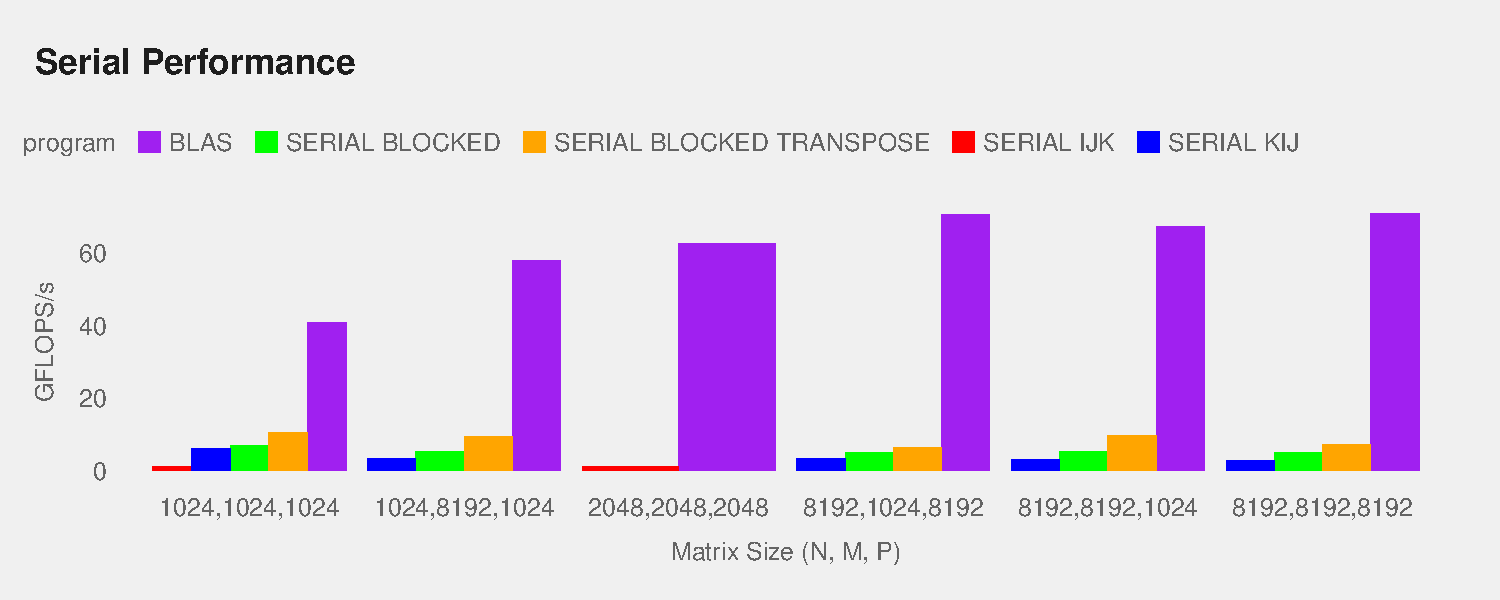
\includegraphics[width=0.8\textwidth]{../../project/out/serial-gflops.pdf}
    \caption{Performance of Serial Code vs. Intel MKL \texttt{dgemm} in GFLOPs/s}
    \label{FIG:SERIAL-GFLOPS} 
\end{figure}

\begin{figure}[H]
    \centering
    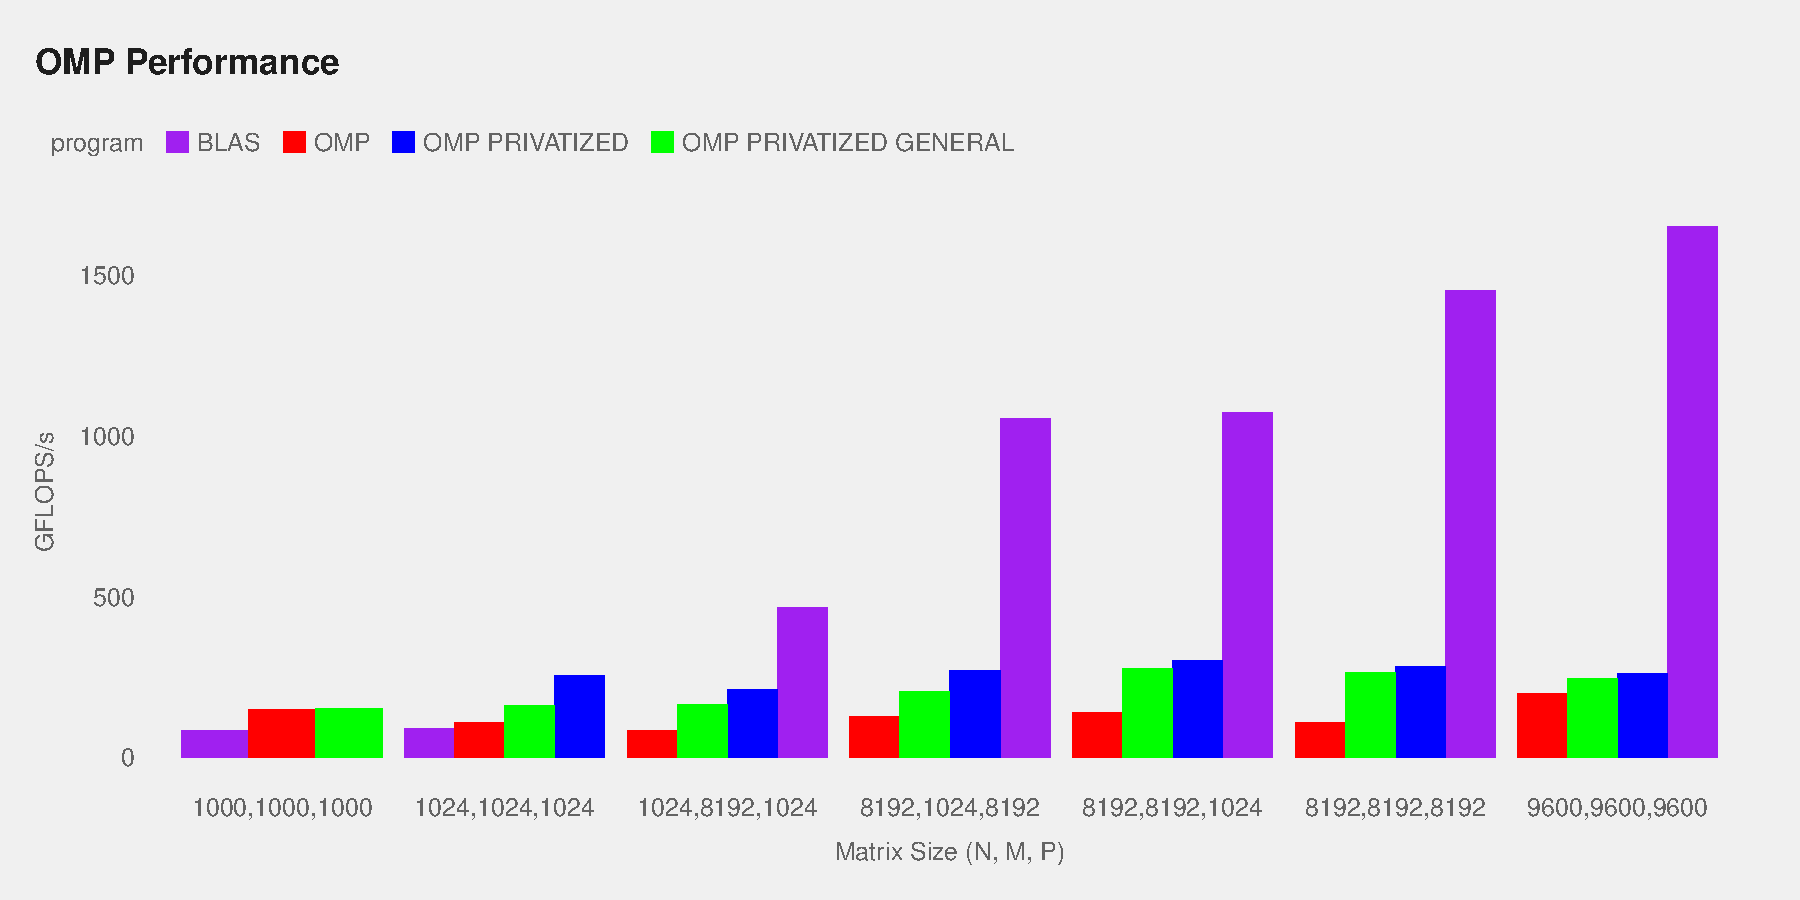
\includegraphics[width=0.8\textwidth]{../../project/out/omp-gflops.pdf}
    \caption{Performance of Multithreaded Code vs. Intel MKL \texttt{dgemm} in GFLOPs/s}
    \label{FIG:OMP-GFLOPS}
\end{figure}
\noindent There is still a lot of room for improvement in both cases. At this point, we have exhausted the suggestions from the video and
must turn to the literature to understand how to improve our code further.

\section{Approach 3: Better Blocking and AVX Instructions}
The papers `Anatomy of High-Performance Matrix Multiplication' \cite{ANATOMY} and 
`The Anatomy of High-Performance Many Threaded Matrix Multiplication' \cite{6877334}
were used as references for further improvement. The main idea is to utilize more efficient 
blocking so that the matrix multiplication streams data from memory to the CPU registers
more efficiently, from which we use AVX-512 instructions to perform the multiply. Since 
we have three layers of cache, we perform hierarchical blocking, i.e., 
we partition matrices into blocks that can reside in \texttt{L3}, from which we 
partition into blocks that can reside in \texttt{L2}, from which we 
partition into blocks that can fit in \texttt{L1}, from which we load effectively into the registers. This optimization 
is highly dependent on the CPU architecture, and so we hard code the optimal block sizes
for our CPU. To handle general matrix dimensions, we pad the matrices to be multiples of the
optimal block size. We continue with the general matrix multiplication between 
$A$ and $B$, where $A$ is $N \times P$ and $B$ is $P \times M$.
\newpage
\subsection{A new Way of Blocking}
\noindent The main idea from the papers is to block as follows:
\begin{lstlisting}
    for (size_t jc = 0; jc < M; jc += NC)
        for (size_t pc = 0; pc < P; pc += KC)
            for (size_t ic = 0; ic < N; ic += MC)
                for (size_t jr = 0; jr < NC; jr += COL_BLOCK)
                    for(size_t ir = 0; ir < MC; ir += ROW_BLOCK)
                        // matrix multiplication kernel to compute C[i][j]
                        // where i and j range from
                        // i -> ir: ir + ROW_BLOCK - 1
                        // j -> jr: jr + COL_BLOCK - 1
\end{lstlisting}
Parroting \cite{6877334}:
\begin{enumerate}
    \item The \texttt{jc} loop partitions $C$ and $B$ into wide column panels.
    \item $A$ and the current column panel of $B$ are partitioned into column panels and row panels, respectively.
    The current width \texttt{NC} column panel of $C$ is updated as a sequence of rank-\texttt{KC} updates, indexed by \texttt{pc}.
    \item The current row panel of $B$ is packed into a contiguous buffer, $\widetilde{B}$, that is kept in \texttt{L3} cache ($\texttt{KC} \times \texttt{NC}$ fits in \texttt{L3}).
    \item The current panel of $A$ is partitioned into blocks indexed by \texttt{ic}. The blocks are packed into another contiguous buffer, $\widetilde{A}$, that is kept in \texttt{L2} cache ($\texttt{MC} \times \texttt{KC}$ fits in \texttt{L2}).
    \item Next, $\widetilde{B}$ is partitioned into column slivers (indexed by \texttt{jr}) of width \texttt{COL\_BLOCK}. At a typical point in the multiply, this sliver resides in the \texttt{L1} cache and multiplies $\widetilde{A}$ (\texttt{KC} * \texttt{COL\_BLOCK} fits in \texttt{L1}). The panel 
    $\widetilde{B}$ was packed so that the sliver in \texttt{L1} cache is contiguous in memory, one row of width \texttt{COL\_BLOCK} at a time. Denote this individual sliver of width \texttt{COL\_BLOCK} by $\widetilde{B}_{jr}$.
    \item Lastly, $\widetilde{A}$ is partitioned into row slivers (indexed by \texttt{ir}) of height \texttt{ROW\_BLOCK}. The block $\widetilde{A}$ was packed so that this sliver is stored contiguously, one column of height \texttt{ROW\_BLOCK} at a time. 
    Denote this individual sliver of height \texttt{ROW\_BLOCK} by $\widetilde{A}_{ir}$.
    \item The multiplication kernel multiplies $\widetilde{A}_{ir}$ and $\widetilde{B}_{jr}$ and updates the current \texttt{ROW\_BLOCK} $\times$ \texttt{COL\_BLOCK} column panel of $C$. The kernel is implemented to perform updates with 
    columns from $\widetilde{A}_{ir}$ and rows from $\widetilde{B}_{jr}$.
\end{enumerate}
This sets up efficient cache utilization. At any point in the computation:
\begin{itemize}
    \item a \texttt{ROW\_BLOCK} $\times$ \texttt{COL\_BLOCK} block of $C$ resides in registers.
    \item the $\texttt{KC} \times \texttt{COL\_BLOCK}$ sliver of $\widetilde{B}$ is in the \texttt{L1} cache.
    \item the $\texttt{ROW\_BLOCK} \times \texttt{KC}$ sliver of $\widetilde{A}$ is in the \texttt{L2} cache and is streamed efficiently during the computation.
\end{itemize}
A very helpful visualization of this process can be seen in the right-most 
animation of \MYhref{https://jukkasuomela.fi/cache-blocking-demo/}{this animated HTML page}.

\subsection{Back to Serial}
Given this new mechanism for blocking, we implement a serial kernel to perform each \texttt{ROW\_BLOCK} $\times$ \texttt{COL\_BLOCK} block of $C$. 
Since we are doing double precision matrix multiplication, we found the best performance when:
\begin{lstlisting}
size_t NC = M           // set to number of columns of B - KC * NC fits in L3
#define KC 240          // KC * COL_BLOCK doubles fit in L1, 32K
#define MC 240          // KC * MC doubles fit in L2, 1024k
#define ROW_BLOCK 10    // operate on 10 rows at a time
#define COL_BLOCK 16    // operate on 16 columns at a time
\end{lstlisting}
For the serial kernel, we assumed $M$ was divisible by 16, $N$ by 240, and $P$ by 240. The kernel and AVX instructions are detailed in Appendix A3.
The performance is observable in Table \ref{TAB:AVX-RESULTS-SERIAL}.
\begin{table}[H]
    \centering
    \caption{AVX Kernel Serial Performance (s)}
    \begin{tabular}[t]{rrrrr}
    \toprule
    N & P & M & Mean Time & Mean Blas Time\\
    \midrule
    1200 & 1200 & 1200 & 0.060 & 0.059\\
    \addlinespace
    1440 & 1440 & 1440 & 0.104 & 0.059\\
    \addlinespace
    1440 & 8160 & 9648 & 4.321 & 1.206\\
    \addlinespace
    3600 & 3600 & 3600 & 1.591 & 0.678\\
    \addlinespace
    4320 & 4320 & 4320 & 2.809 & 1.038\\
    \addlinespace
    8400 & 8400 & 8400 & 20.384 & 4.941\\
    \addlinespace
    9600 & 9600 & 9600 & 31.710 & 12.313\\
    \bottomrule
    \end{tabular}
    \label{TAB:AVX-RESULTS-SERIAL}
\end{table}
\noindent We observe similar performance for small sized matrices and note the performance of MKL's \texttt{dgemm} 
still outperforms the serial implementation by a significant margin. Assessing the performance in GFLOPS/s 
is done in Figure \ref{FIG:AVX-SERIAL-GFLOPS}.

\begin{figure}[H]
    \centering
    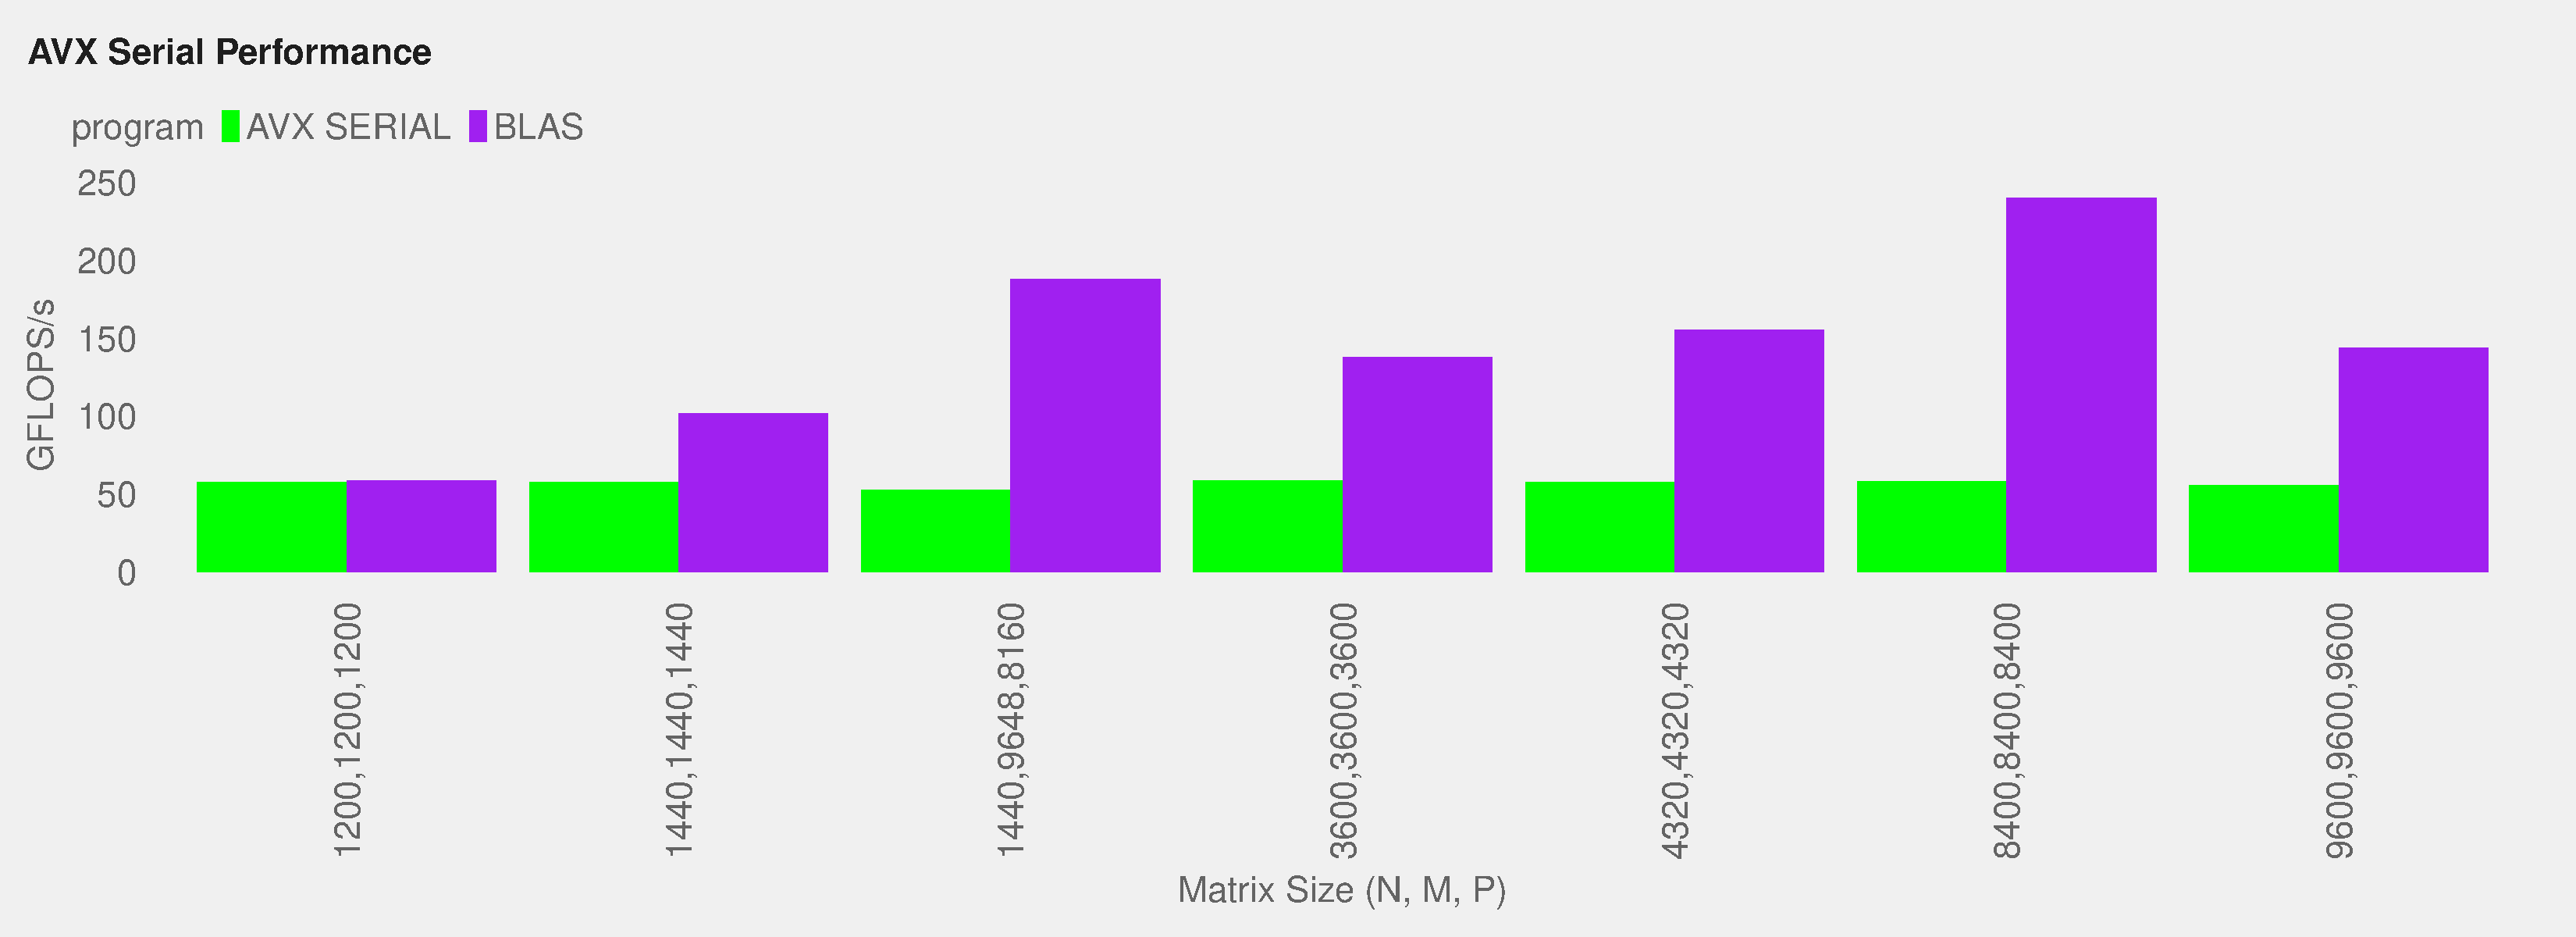
\includegraphics[width=0.8\textwidth]{../../project/out/avx-serial-gflops.pdf}
    \caption{Performance of AVX Serial Code vs. Intel MKL \texttt{dgemm} in GFLOPs/s}
    \label{FIG:AVX-SERIAL-GFLOPS}
\end{figure}
\noindent There is likely some more clever utilization of the cache that can be done for a single core. 
We now turn to the multithreaded case.

\subsection{Multithreading}
The serial code is now parallelized with OpenMP. Choosing which loop to parallelize requires careful consideration. 
As structured, the \texttt{jc} loop is only 1 iteration, while the \texttt{pc} and \texttt{ic} loops have 
a negligible amount of iterations compared to the \texttt{ir} and \texttt{jr} loops. It 
was found that parallelizing the \texttt{jr} loop yielded the highest performance and thus only the \texttt{jr} loop is parallelized.\footnote{Some non recorded experiments were done to collapse the 5 loops, but this did not improve performance.}

\

\noindent The results are shown in Table \ref{TAB:AVX-RESULTS-OMP} and Figure \ref{FIG:AVX-OMP-GFLOPS}.
\begin{table}[H]
    \centering
    \caption{AVX Kernel Serial Performance (s)}
    \begin{tabular}[t]{rrrrr}
    \toprule
    N & P & M & Mean Time & Mean Blas Time\\
    \midrule
    1200 & 1200 & 1200 & 0.006 & 0.052\\
    \addlinespace
    1440 & 1440 & 1440 & 0.010 & 0.031\\
    \addlinespace
    1440 & 8160 & 9648 & 0.219 & 0.437\\
    \addlinespace
    3600 & 3600 & 3600 & 0.115 & 0.100\\
    \addlinespace
    4320 & 4320 & 4320 & 0.193 & 0.148\\
    \addlinespace
    8400 & 8400 & 8400 & 1.051 & 0.776\\
    \addlinespace
    9600 & 9600 & 9600 & 1.605 & 1.165\\
    \bottomrule
    \end{tabular}
    \label{TAB:AVX-RESULTS-OMP}
\end{table} 
\noindent We observe a significant improvement over the serial case. For $M = N = P = 9600$, the performance
improves by a factor of 19.8 as opposed to the 10.5 times improvement of BLAS. 
The performance in GFLOPS/s is shown in Figure \ref{FIG:AVX-OMP-GFLOPS}.
\begin{figure}[H]
    \centering
    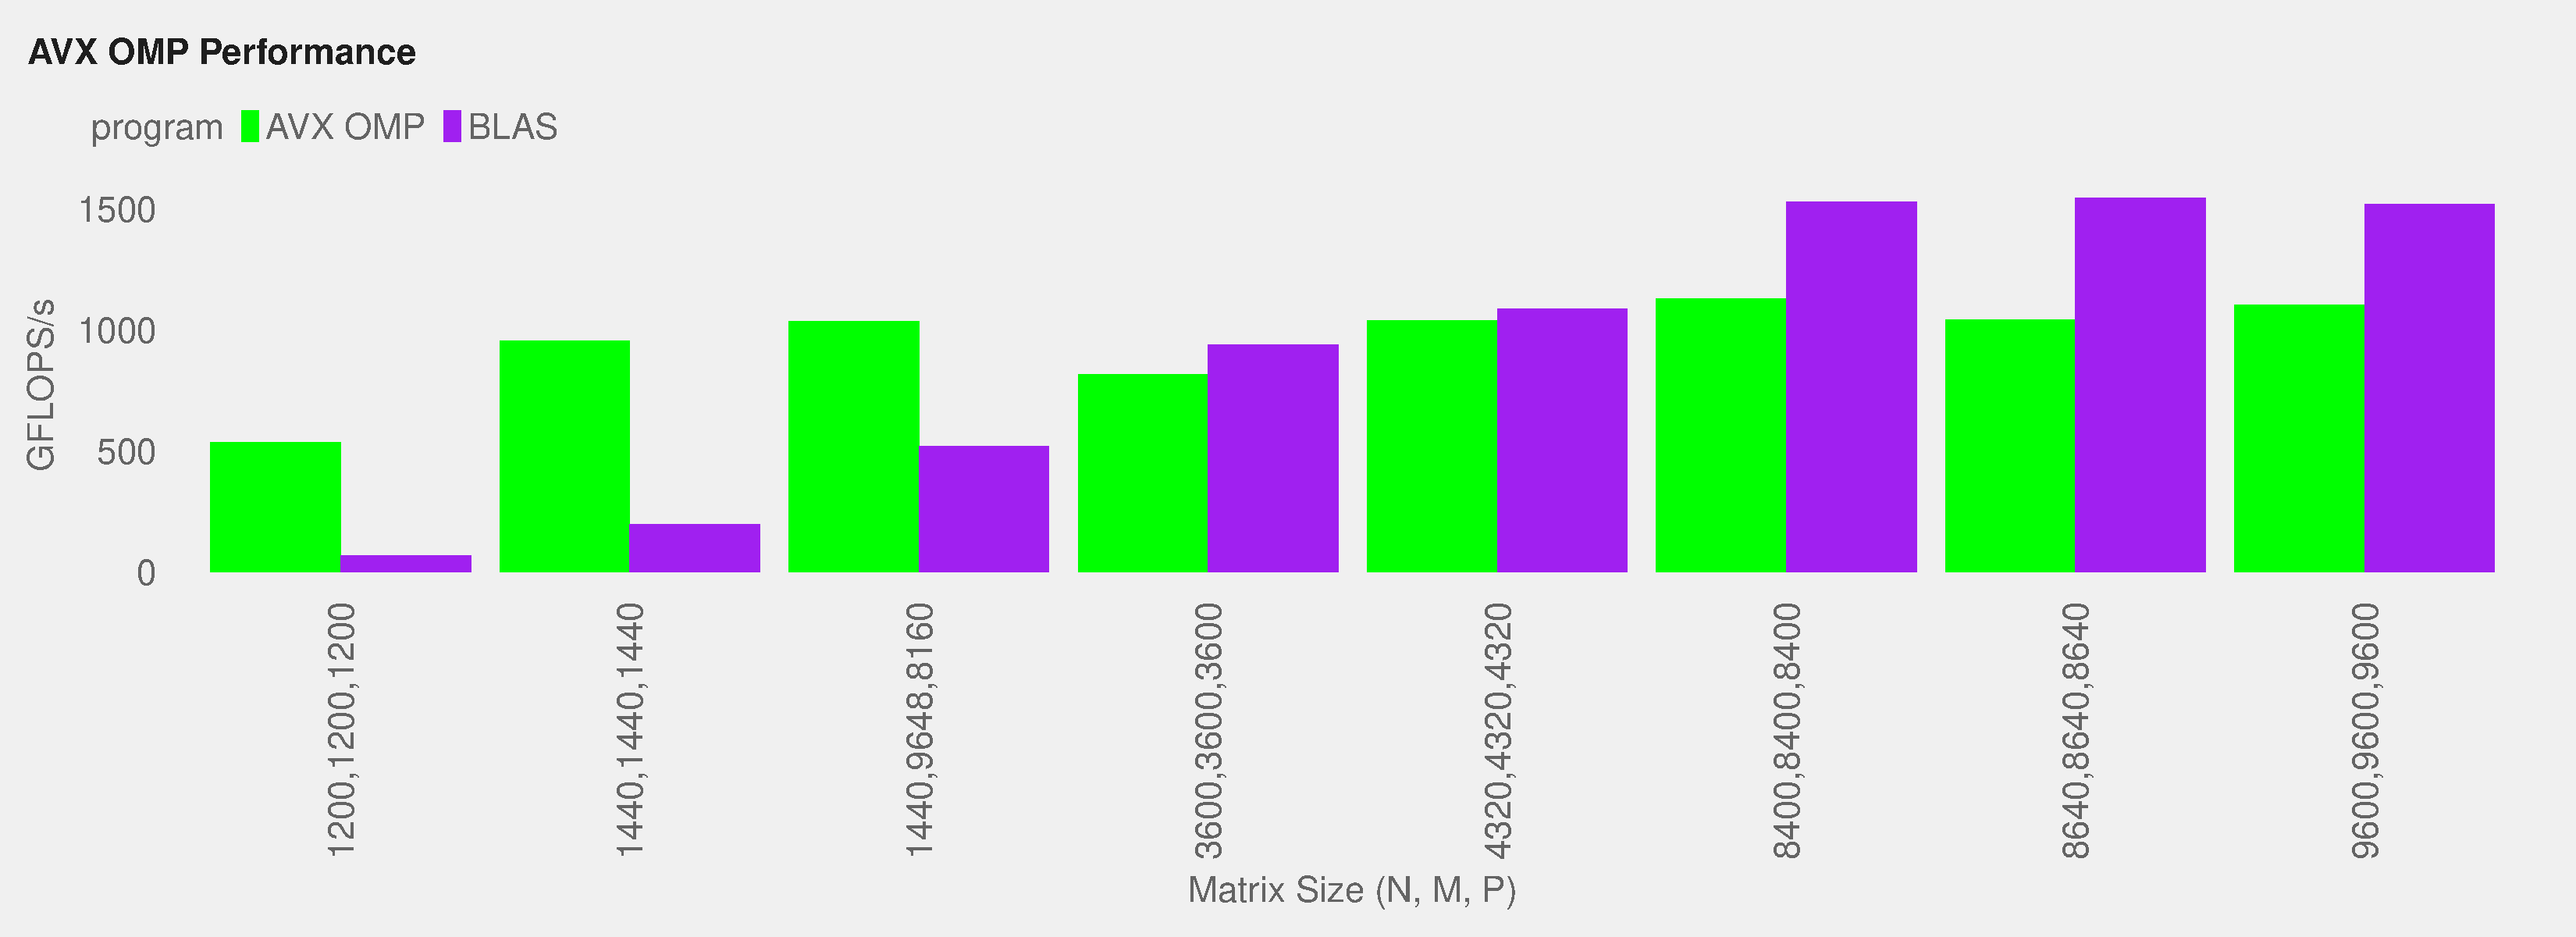
\includegraphics[width=0.95\textwidth]{../../project/out/avx-omp-gflops.pdf}
    \caption{Performance of AVX Multithreaded Code vs. Intel MKL \texttt{dgemm} in GFLOPs/s}
    \label{FIG:AVX-OMP-GFLOPS} 
\end{figure}

\

\noindent It should be noted that this performance is a bit misleading as a direct comparitor to \texttt{dgemm} 
since it does not handle all matrix sizes. The general implementation was also implemented and the results are 
shown in figure \ref{FIG:AVX-OMP-GENERAL-GFLOPS}. The performance is slightly worse than 
the non general implementation, but still significantly better than the serial case. The tradeoff of 
having to pad the matrices is worth it for the generalizability of the code.

\begin{figure}[H]
    \centering
    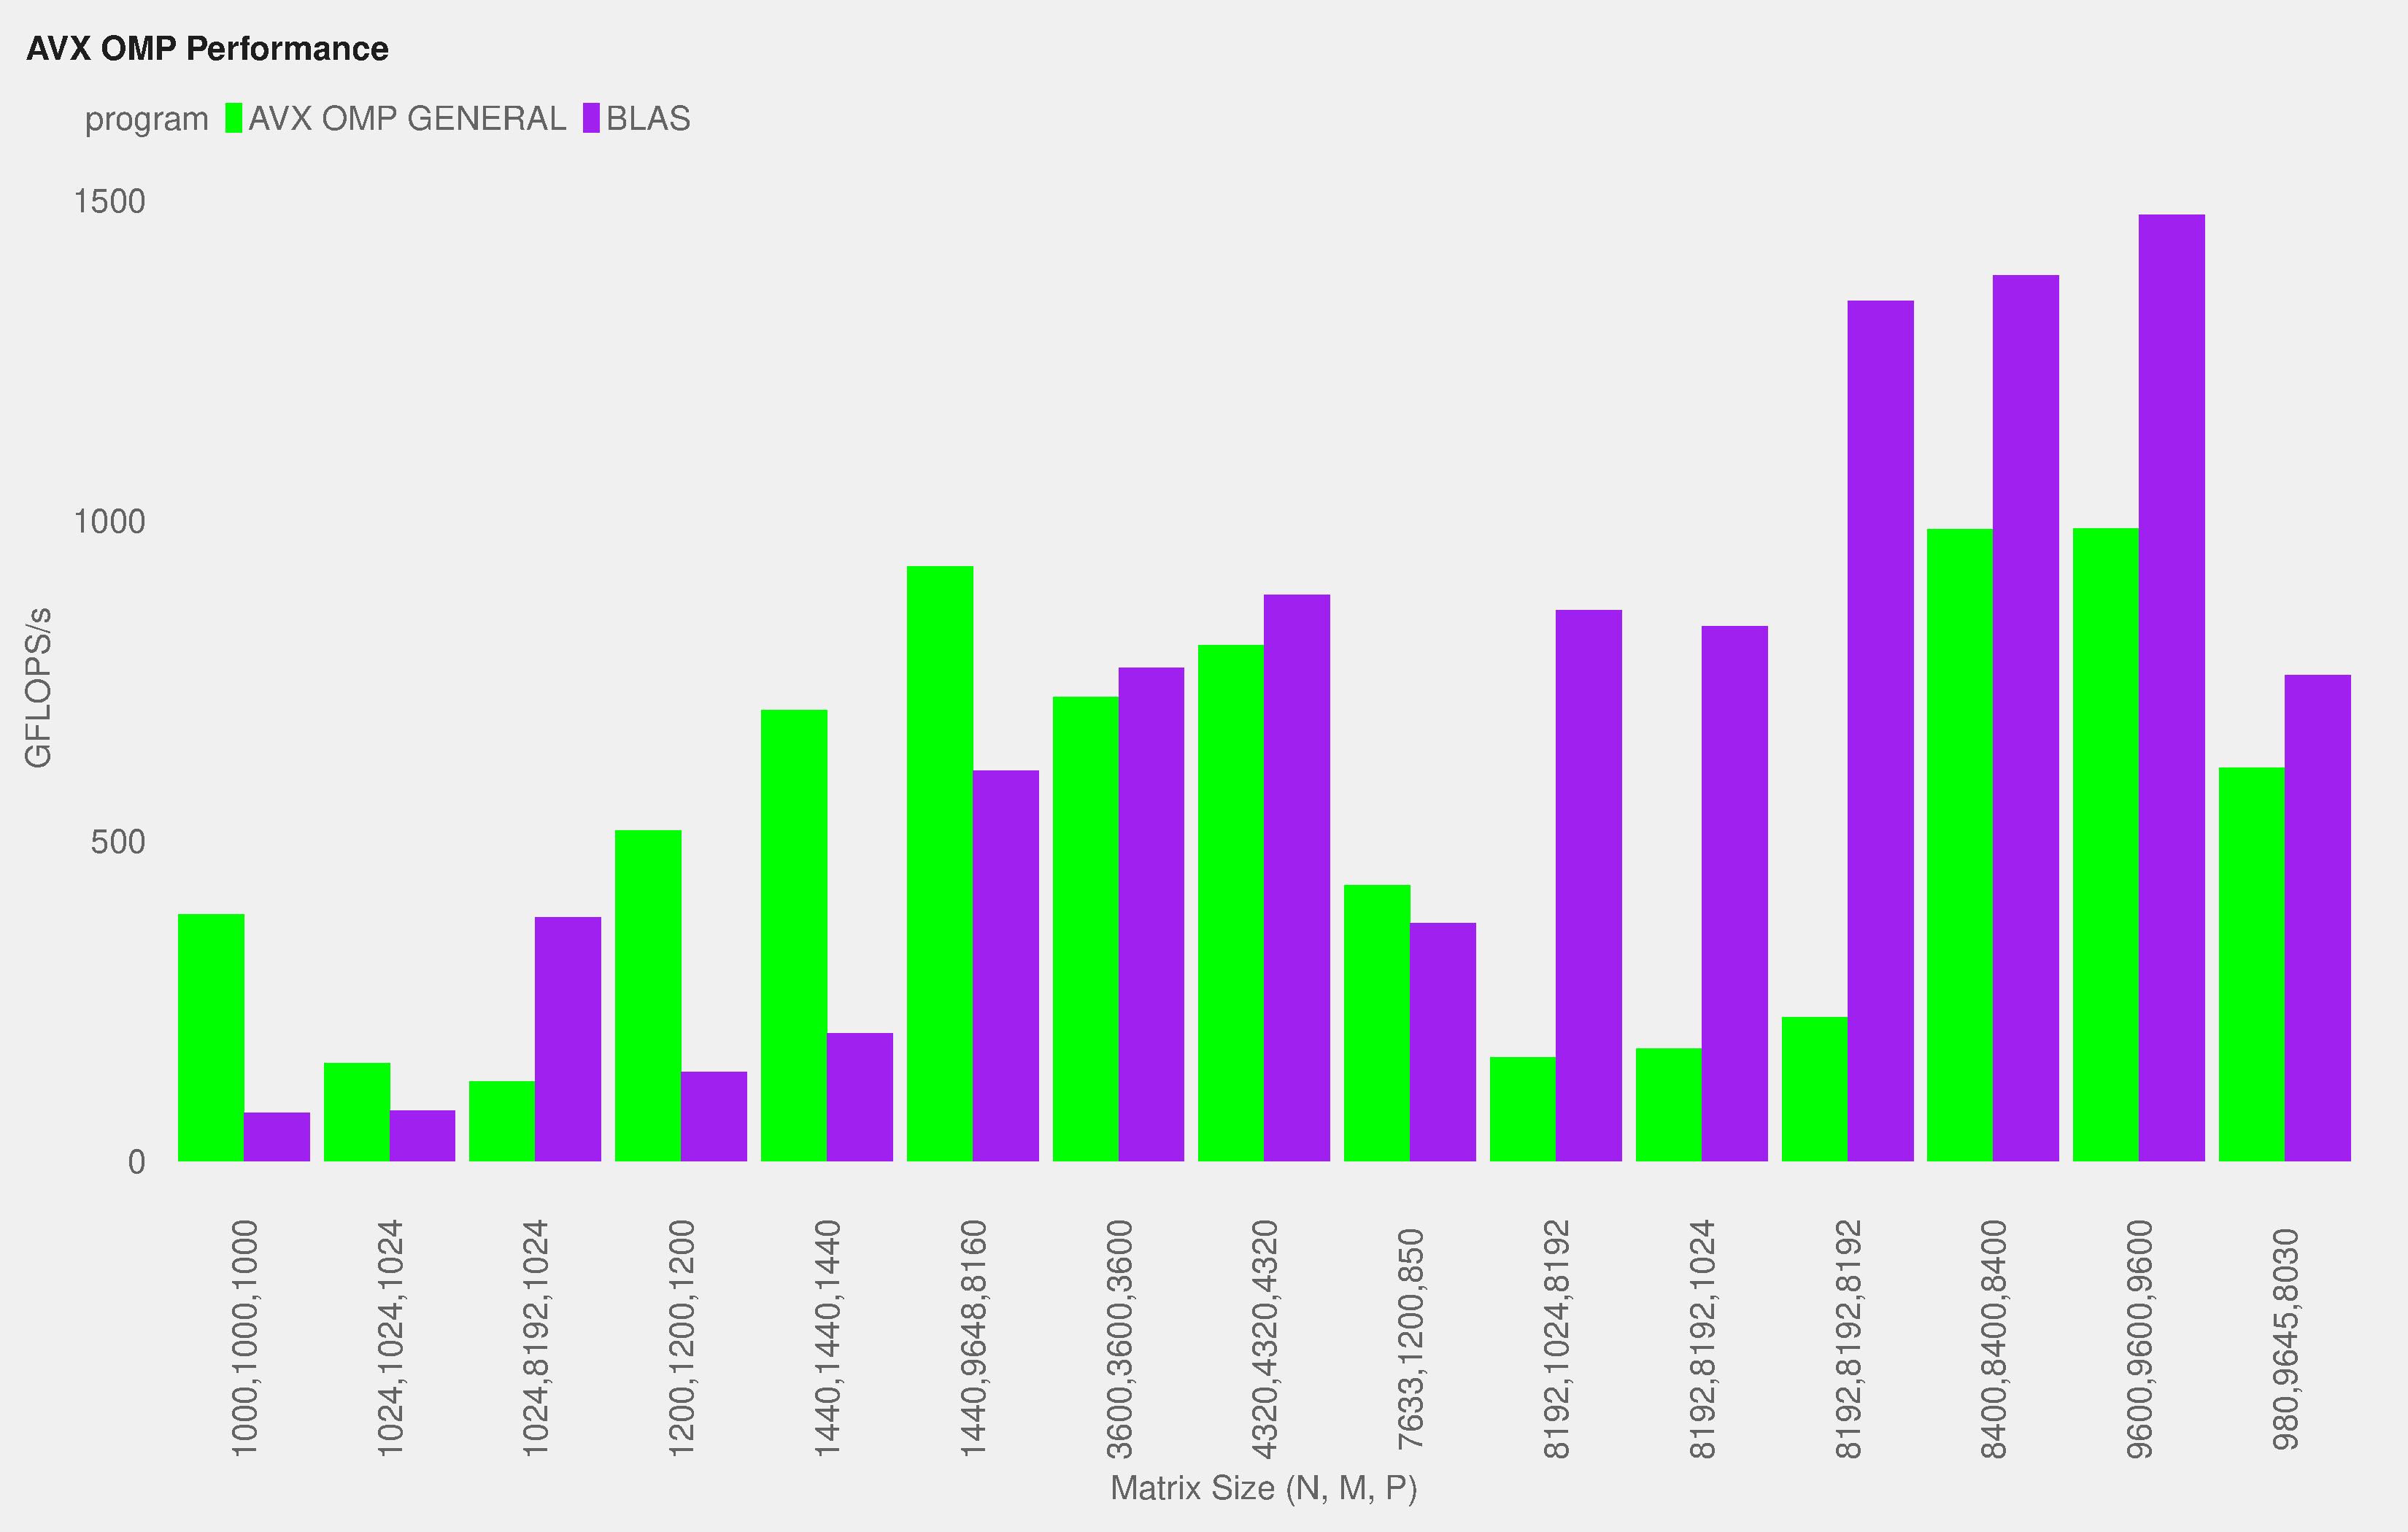
\includegraphics[width=0.8\textwidth]{../../project/out/avx-omp-non-divisible-gflops.pdf}
    \caption{Performance of AVX Multithreaded Code vs. Intel MKL \texttt{dgemm} in GFLOPs/s}
    \label{FIG:AVX-OMP-GENERAL-GFLOPS}
\end{figure}

\subsection{Assessment}
The adoption of hierarchical blocking in conjunction with AVX instructions has 
led to significant performance gains in matrix multiplication, particularly when utilizing the capabilities 
of multiple cores. The results obtained from both the serial and multithreaded implementations demonstrate 
substantial improvements over the initial approaches, underscoring the power of proper cache utilization.

\paragraph*{Hierarchical Blocking Efficiency} The hierarchical blocking approach, 
aligning with the L1, L2, and L3 cache sizes, has shown to be highly effective. 
By partitioning matrices into blocks that fit well within the cache hierarchy, 
the algorithm has minimized cache misses and maximized cache utilization. 
This optimization is particularly evident in large matrix sizes, where managing the cache behavior is crucial for performance.

\paragraph*{Impact of AVX Instructions} The use of AVX-512 instructions was pivotal 
in enhancing computational efficiency. By enabling simultaneous operations on multiple data points, 
these instructions have drastically increased the throughput of the matrix multiplication operation. 
The results, especially in the multithreaded context, highlight the potential of AVX instructions in harnessing 
the full computational power the CPU.

\paragraph*{Comparison with MKL's \texttt{dgemm}} While the MKL's \texttt{dgemm} implementation 
remains a tough competitor, especially for larger matrices, 
the gap in performance has been considerably narrowed. For smaller matrices, the performance 
of the optimized algorithm is on par with \texttt{dgemm}, and even for larger matrices, 
the algorithm shows competitive performance, especially considering the inherent challenges in achieving such optimization levels 
without the backing of a billion dollar publicly traded company.

\section{Conclusion}
This project embarked on a comprehensive exploration of optimizing matrix multiplication on CPUs, 
motivated by a quest to match the performance of BLAS, particularly Intel's Math Kernel Library (MKL) 
implementation of \texttt{dgemm}. The journey traversed through various stages of optimization, 
each progressively edging closer to the goal of achieving high performance on CPU architectures.

\

\noindent Initially, the project delved into the nuances of matrix multiplication as a compute-bound task, 
highlighting the impact of memory access patterns and computational intensity. The exploration began 
with serial implementations, starting from a naive \texttt{ijk} algorithm, progressing to 
loop reordering for better cache efficiency, and eventually adopting a blocking strategy. 
Each step yielded valuable insights into how memory access and data locality profoundly influence performance.

\

\noindent The project then ventured into the realm of parallel computing with OpenMP, 
leveraging the power of multi-core processors. This phase demonstrated the scalability of matrix multiplication 
algorithms and the effectiveness of multithreading in reducing computation time. However, it also revealed the intricacies 
of parallel programming, such as addressing false sharing, and the need for carefully considering data privatization to 
avoid performance degradation.

\

\noindent Further advancements were made by incorporating AVX instructions, aligning with the processors capabilities to 
execute multiple floating-point operations simultaneously. This approach required a deeper understanding of CPU architecture, 
leading to the implementation of hierarchical blocking that aligns with the cache hierarchy of the CPU. The results from 
this stage brought us significantly closer to the performance of MKL's \texttt{dgemm}, especially in the multithreaded context.

\

\noindent In conclusion, this project has demonstrated that, while challenging, it is possible to significantly optimize 
matrix multiplication on CPUs. The key lessons learned revolve around the 
importance of understanding the underlying hardware, the role of memory access patterns, 
and the effective use of parallel computing techniques. While the performance of MKL's \texttt{dgemm} remains a 
high (very proprietary) bar, the progress made in this report showcases the potential 
and feasibility of optimizing matrix multiplication on CPUs to a level that rivals highly specialized libraries. 
As CPU architectures continue to evolve, so too will the strategies and techniques for optimizing matrix multiplication, 
an operation fundamental to many fields in computational science.

\newpage
\section{Appendix A1: Project Organization}
The project is laid out as follows:
\begin{multicols}{2}
    \begin{forest}
        for tree={
            font=\ttfamily,
            grow'=0,
            child anchor=west,
            parent anchor=south,
            anchor=west,
            calign=first,
            edge path={
                \noexpand\path [draw, \forestoption{edge}]
                (!u.south west) +(7.5pt,0) |- node[fill,inner sep=1.25pt] {} (.child anchor)\forestoption{edge label};
            },
            before typesetting nodes={
                if n=1
                {insert before={[,phantom]}}
                {}
            },
            fit=band,
            before computing xy={l=15pt},
        }
    [
        [docs/]
        [bin/]
        [out/]
        [src/
        [1-serial/]
        [2-omp/]
        [3-avx/]
        ]
        [Makefile-serial]
        [Makefile-omp]
        [Makefile-avx]
    ]
    \end{forest}
    \columnbreak
    \begin{itemize}
        \item \textbf{docs/}: This folder contains LaTeX files and other documentation materials that pertain to the report.
        \item \textbf{bin/}: The \texttt{bin} folder holds compiled objects and executable files, centralizing the output of the compilation process.
        \item \textbf{out/}: The \texttt{out} folder stores the outputs from each task. It also houses the csv file containing data generated by the programs.
        \item \textbf{src/}: This directory houses the source files (\texttt{.c}) that make up the benchmarks. Each subdirectory contains the source files for the relevant 
        experiments.
        \item \textbf{Shell Scripts}: The shell scripts are used to submit the job for the relevant task to slurm via \texttt{sbatch}.  
        \item \textbf{Makefiles}: The Makefiles are used to compile the code. There is a Makefile for each set of experiments. The relevant shell scripts make use 
        of the appropriate Makefile.
    \end{itemize}
\end{multicols}
\newpage
\section{Appendix A2: Code Explanation, Compilation, and Execution}

The provided Bash scripts automate the entire process, 
making it straightforward to compile and run the code. All the below steps assume 
you are in the root of the project directory.

\subsection{Automated Building and Execution}
All related code is in the \texttt{src/} directory.
There are multiple programs, each batch of which is contained in its own subdirectory.
\subsubsection*{Serial Programs}
\begin{itemize}
    \item \texttt{t1-serial-ijk.c}: Standard serial matrix multiplication.
    \item \texttt{t2-serial-kij.c} Serial matrix multiplication algorithm with better cache performance.
    \item \texttt{t3-serial-blocking.c} Serial tiled matrix multiplication.
    \item \texttt{t4-serial-blocking-T.c} Serial tiled matrix multiplication where $B$ is transposed.
\end{itemize}

\subsubsection*{Open MP Programs}
\begin{itemize}
    \item \texttt{t5-omp.c}: Utilized OpenMP to parallelize the serial matrix multiplication algorithm in \texttt{t4}.
    \item \texttt{t6-omp-divisible-local-blocks.c}: Fixes the false sharing problem in \texttt{t5}: which is when 
    multiple cores are accessing the same cache line on the shared cache. This program assumes 
    matrix dimensions are multiples of the chosen block (tile) size.
    \item \texttt{t7-omp-non-divisible-local-blocks.c}: Same as \texttt{t6} but does not assume matrix dimensions are multiples of the chosen block size.
\end{itemize}

\subsubsection*{AVX Programs}
These programs are inspired by \cite{6877334}, \cite{ANATOMY}, and \cite{BLAS-P}.
\begin{itemize}
    \item \texttt{t8-serial-divisible-avx-blocking.c}: Serial matrix multiplication with AVX instructions. This program assumes
    that the matrix dimensions are multiples of the hard coded optimal block sizes.
    \item \texttt{t9-omp-divisible-avx-blocking.c}: Parallel matrix multiplication with OpenMP and AVX instructions. This program assumes
    that the matrix dimensions are multiples of the hard coded optimal block sizes.
    \item \texttt{t10-omp-non-divisible-avx-blocking.c}: Parallel matrix multiplication with OpenMP and AVX instructions. This program does not assume
    anything about the matrix dimensions and can handle non-multiples of the hard coded optimal block sizes.
\end{itemize}

\noindent To run any one set of experiments, simply run the relevant Bash script. For example, to run the serial experiments, submit the \texttt{build-run-serial.sh}
script via \texttt{sbatch}: \texttt{sbatch build-run-serial.sh}. This will compile the code and run the experiments. The output files will be stored in the \texttt{out/} directory.

\subsection{Post-Build Objects and Executables}
Upon successful compilation and linking, an \texttt{obj/} subdirectory will be generated within the directory. 
This directory will contain the compiled output files. Additionally, the executable files for running each program will be 
situated in the \texttt{bin/} subdirectory.

\subsection{Output Files From \texttt{sbatch}}
The output files generated from running the code by submitting the relevant Bash script via \texttt{sbatch} will be 
stored in the \texttt{out} directory. 
\newpage
\section{Appendix A3: AVX Kernel}
This is a simplified version of the AVX kernel with \texttt{ROW\_BLOCK} set to 2 for demonstration purposes. 
The \texttt{COL\_BLOCK} is set to 16 so each update of $C$ is 2 rows $\times$ 16 columns at a time. 
\begin{lstlisting}
    // 512 bit wide registers (operate on 8 doubles at once)
    __m512d mB0, mB1, mA0, mA1;
    
    // 2 x 16 block of C in registers
    __m512d result0_0 = _mm512_set1_pd(0); // 1 x 8 (first 8 doubles of row 0)
    __m512d result1_0 = _mm512_set1_pd(0); // 1 x 8 (first 8 doubles of row 1)

    __m512d result0_1 = _mm512_set1_pd(0); // 1 x 8 (second 8 doubles of row 0)
    __m512d result1_1 = _mm512_set1_pd(0); // 1 x 8 (second 8 doubles of row 1)

    for (size_t k = 0; k < KC; k++)
    {
        // load 16 consecutive doubles from k'th row of B (8 to mB0 and 8 to mB1)
        mB0 = _mm512_load_pd(&B[M * (k + pc) + jc + jr]);
        mB1 = _mm512_load_pd(&B[M * (k + pc) + jc + jr + 8]);
    
        // Load a single value for the k'th col of A
        mA0 = _mm512_set1_pd(A[k + pc + (ic + ir) * P]);
        mA1 = _mm512_set1_pd(A[k + pc + (ic + ir + 1) * P]);
    
        // compute 2 x 16 block of C with fmadd instructions
        result0_0 = _mm512_fmadd_pd(mB0, mA0, result0_0);
        result0_1 = _mm512_fmadd_pd(mB1, mA0, result0_1);
        result1_0 = _mm512_fmadd_pd(mB0, mA1, result1_0);
        result1_1 = _mm512_fmadd_pd(mB1, mA1, result1_1);
    }
    
    // store results back in C
    *((__m512d *)(&C[(ic + ir + 0) * M + jc + jr]))             += result0_0;
    *((__m512d *)(&C[(ic + ir + 0) * M + jc + jr + 8]))         += result0_1;
    *((__m512d *)(&C[(ic + ir + 1) * M + jc + jr]))             += result1_0;
    *((__m512d *)(&C[(ic + ir + 1) * M + jc + jr + 8]))         += result1_1;
\end{lstlisting}
The performance of this kernel was maximized for a \texttt{ROW\_BLOCK} of 10 and a \texttt{COL\_BLOCK} of 16 with 
the aforementioned \texttt{KC}, \texttt{MC}, and \texttt{NC} values. 

\newpage
\bibliographystyle{unsrt}
\bibliography{References.bib}

\end{document}
